\ylDisplay{Nöör rennis} % Ülesande nimi
{Stanislav Zavjalov} % Autor
{lahtine} % Voor
{2012} % Aasta
{G 9} % Ülesanne nr.
{9} % Raskustase
{
% Teema: Staatika
\ifStatement
\begin{wrapfigure}{r}{0.4\linewidth}
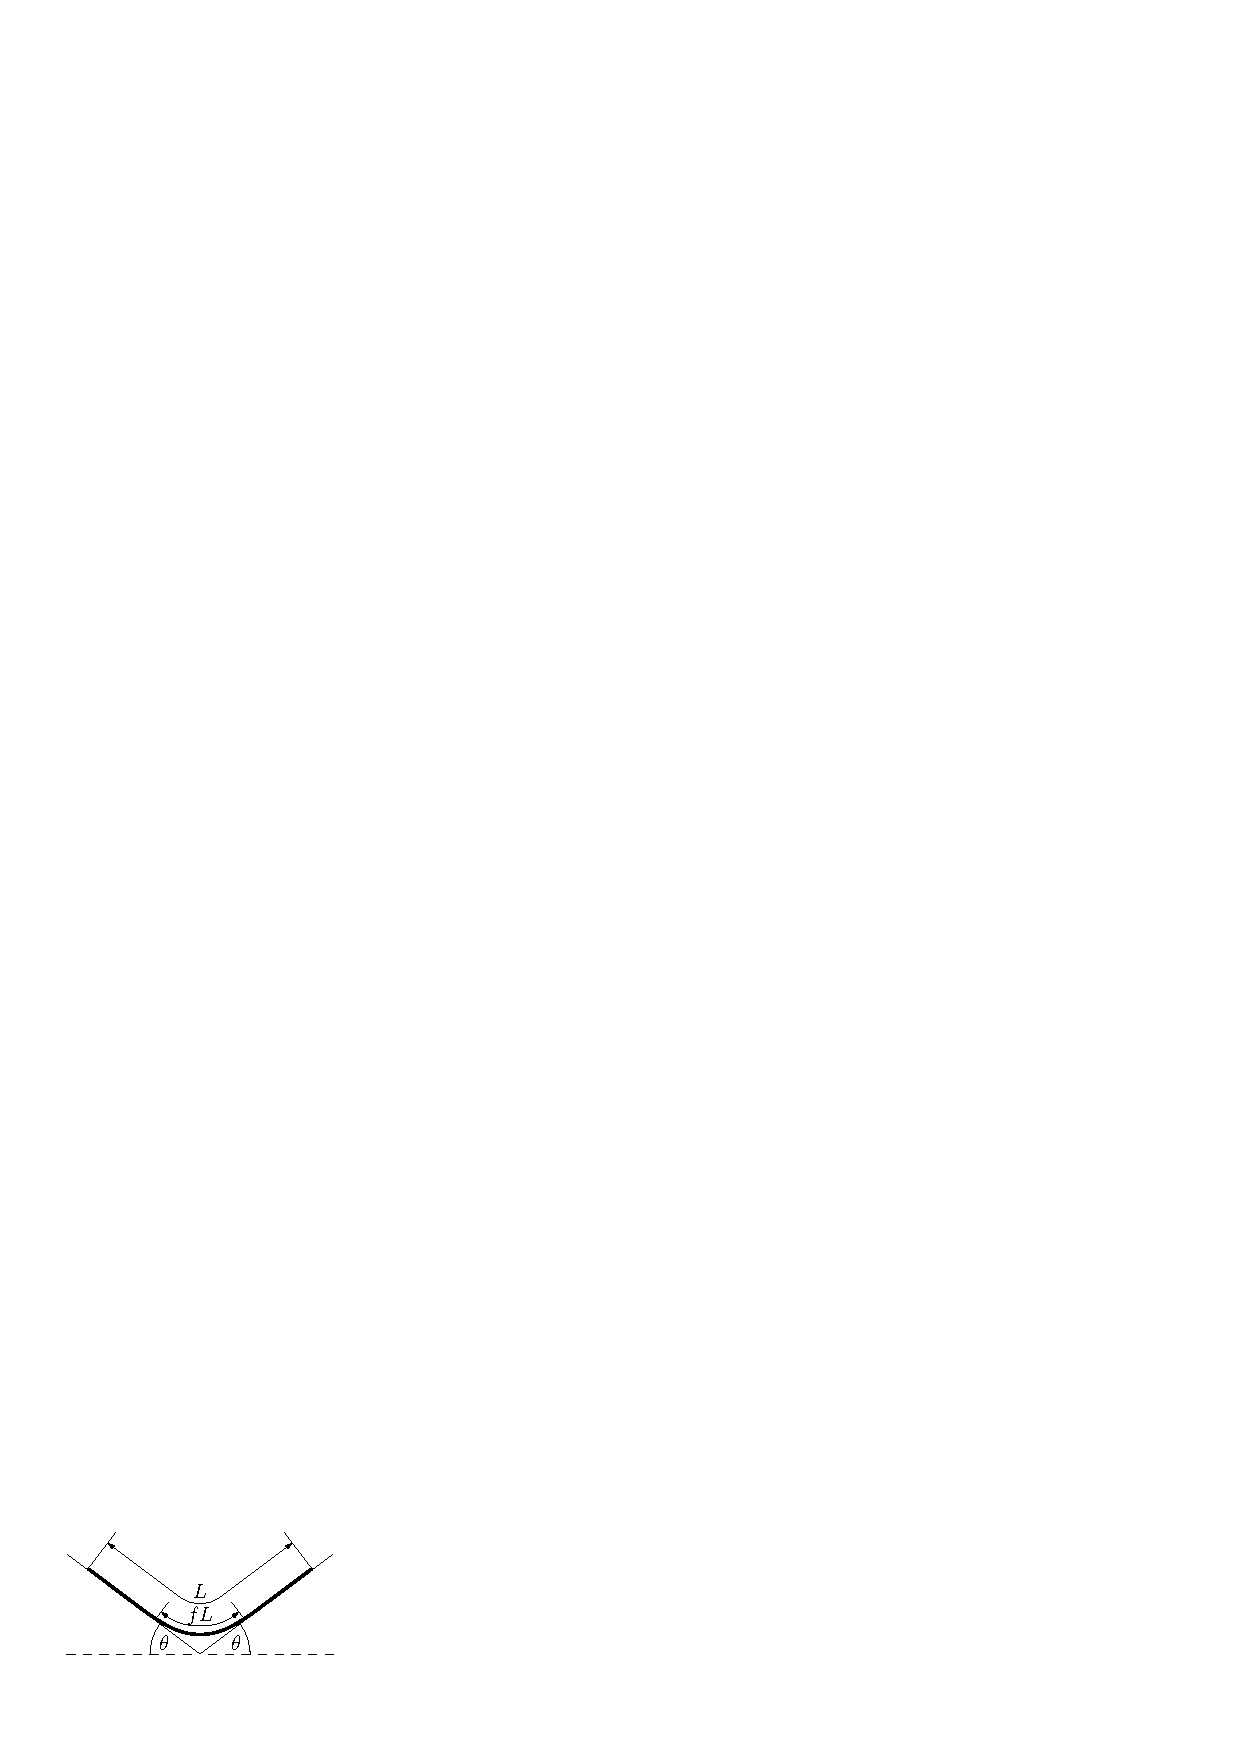
\includegraphics[width=\linewidth]{2012-lahg-09-n88r_ipe}
\end{wrapfigure}
Kaks plaati moodustavad V-kujulise horisontaalse renni. Mõlemad plaadid on
horisontaaltasapinna suhtes nurga $\theta$ all.
Rennis on jupp ühtlase
massijaotusega nööri pikkusega $L$, mis asub tervikuna renniga ristuvas tasandis
nii, et mõlema plaadiga puutub kokku sama palju nööri.
Renni põhja kohal ei toetu nöör enam pikkuse $fL$
ulatuses plaatidele.  Leidke $f$, kui nöör on libisemise piiril. Hõõrdetegur nööri ja plaatide
vahel on $\mu = 1$.
\fi


\ifHint
Nöörile mõjuvad kolm jõudu: raskusjõud, nööri toereaktsioon ning hõõrdejõud. Selleks, et tasakaalutingimusi kirja panna on mugav vaadelda õhus rippuvat osa ja plaadil lebavat osa eraldi. Seejuures peab arvestama ka nööri ja plaadi kokkupuutepunktis mõjuva nööri pingega.
\fi


\ifSolution
Olgu kogu nööri mass $m$. Vaatleme nööri paremat poolt. Nööri pinge vertikaalkomponent nööri ja plaadi kokkupuutepunktis, $T \sin \theta$, peab tasakaalustama õhus rippuva osa kaalu $\frac{f}{2}mg$. Nüüd vaatleme plaadil lebavat osa, selle mass on $\frac{1-f}{2}m$. Seega nii toereaktsioon kui ka maksimaalne hõõrdejõud (kuna $\mu = 1$) on $\frac{1-f}{2}mg \cos \theta$. Hõõrdejõud peab olema tasakaalus raskusjõu komponendiga piki nööri, $\frac{1-f}{2}mg \sin \theta$, ning pingega $T=\frac{f m g}{2 \sin \theta}$: $$\frac{f m g}{2 \sin \theta} + \frac{1-f}{2}mg \sin \theta = \frac{1-f}{2}mg \cos \theta.$$
Siit saame avaldada vastuse $$f = \frac{1-\tan \theta}{1+\tan \theta} \tan \theta. $$
\fi


\ifEngStatement
% Problem name: Rope in groove
\begin{wrapfigure}{r}{0.4\linewidth}
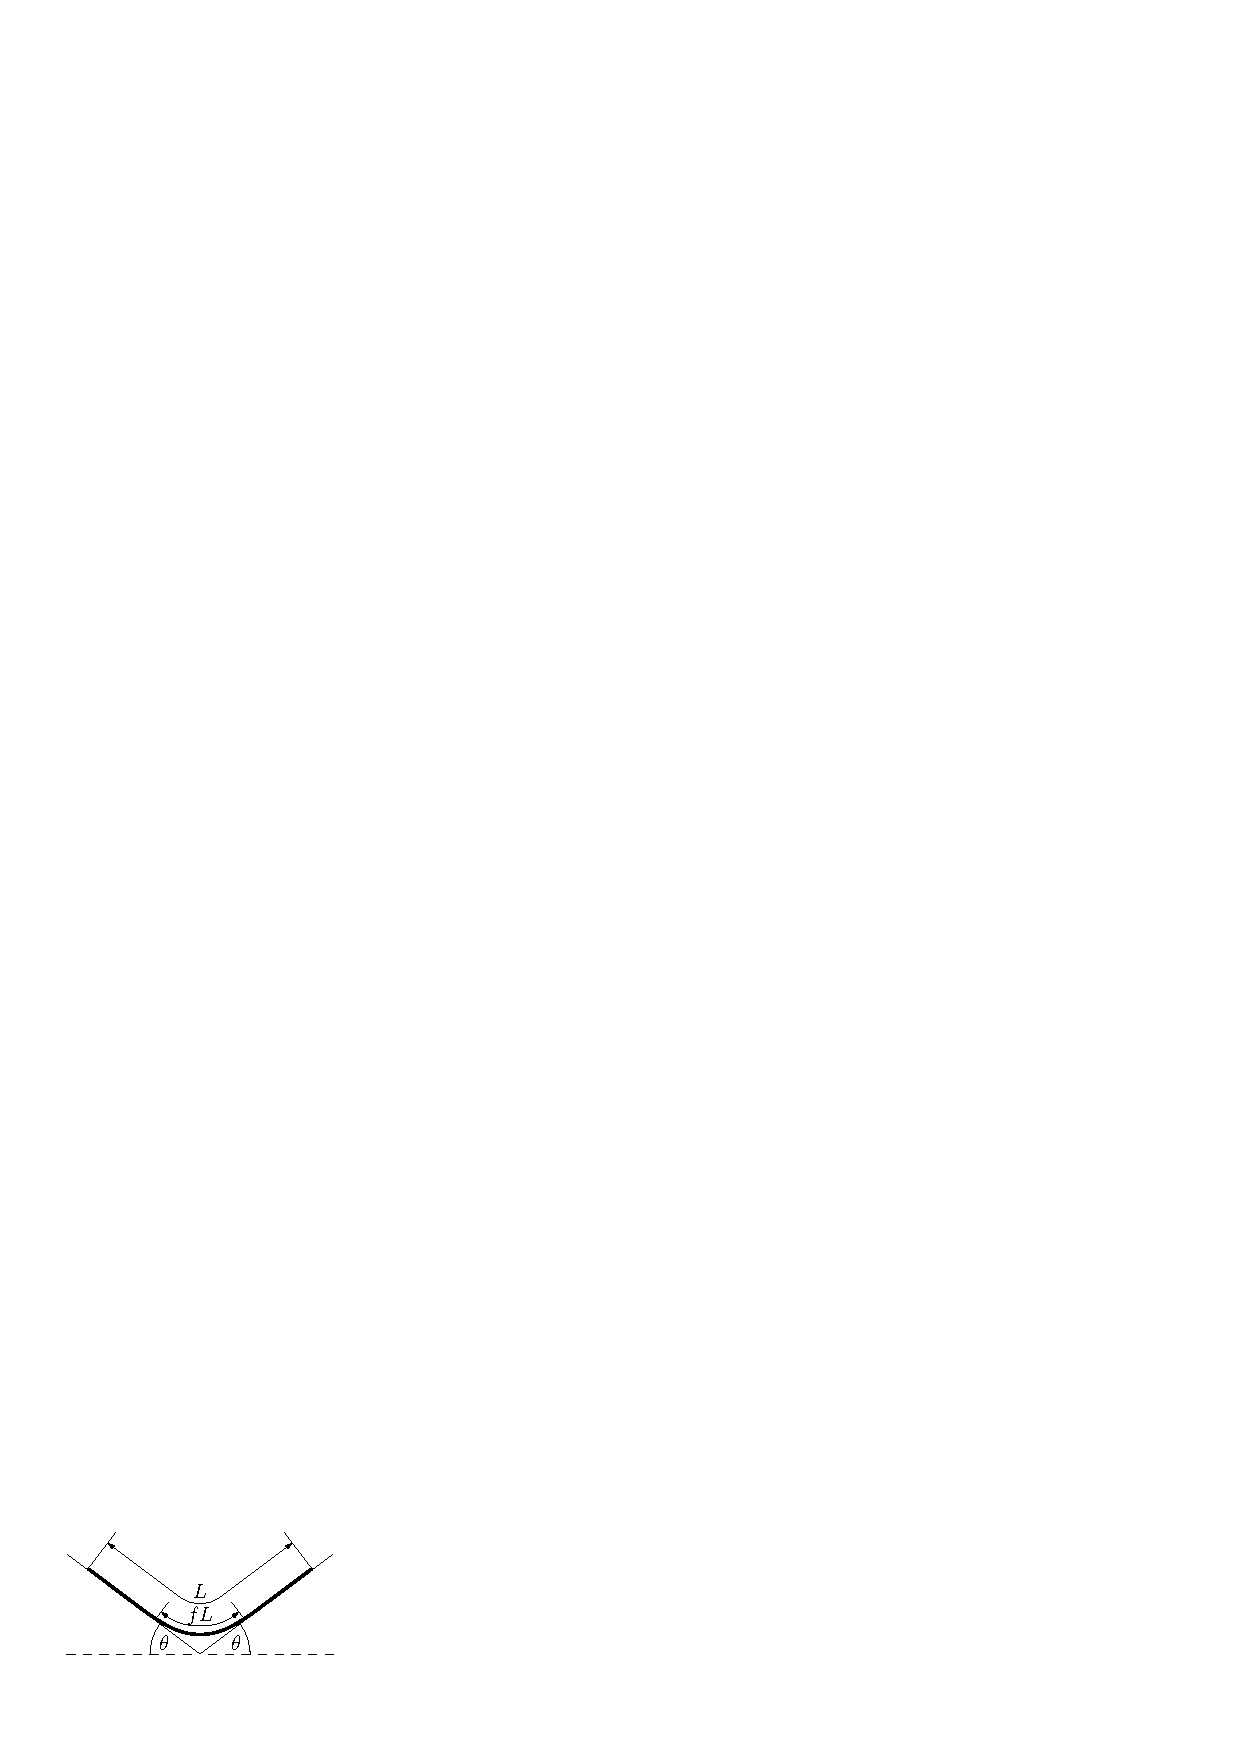
\includegraphics[width=\linewidth]{2012-lahg-09-n88r_ipe}
\end{wrapfigure}
Two plates make up a V-shaped horizontal groove. Both of the plates are at an angle $\theta$ with respect to the ground. In the groove there is a section of rope of length $L$ and of even mass distribution. All of the rope is located on the plane perpendicular to the groove so that both of the plates are touching the same amount of the rope. Above the bottom of the groove a part of the rope of length $fL$ does not anymore rest on the plates. Find $f$ if the rope is on the verge of slipping. The coefficient of friction between the rope and the plates is $\mu = 1$.
\fi


\ifEngHint
Three forces are applied to the rope: gravity force, normal force of the rope and friction force. To write down the equilibrium conditions it is convenient to observe the end hanging in the air and the end lying on the plate separately.  Moreover, you should take into account the tension of the rope that is applied to the contact point of the plate and rope.
\fi


\ifEngSolution
Let the rope’s mass be $m$. Let us observe the rope’s right side. The vertical component of the rope’s tension $T \sin \theta$ at the contact point of the rope and the plate has to balance the weight of the rope hanging in the air, $\frac{f}{2}mg$. Now let us observe the part lying on the plate, its mass is $\frac{1-f}{2}m$. Therefore both the normal force and the maximal friction (because $\mu = 1$) are $\frac{1-f}{2}mg \cos \theta$. The friction has to balance the component of the gravity force along the rope, $\frac{1-f}{2}mg \sin \theta$, and the tension $T=\frac{f m g}{2 \sin \theta}$. 
$$\frac{f m g}{2 \sin \theta} + \frac{1-f}{2}mg \sin \theta = \frac{1-f}{2}mg \cos \theta.$$
From here we can express the answer
$$f = \frac{1-\tan \theta}{1+\tan \theta} \tan \theta. $$
\fi
}